\documentclass[letterpaper,12pt]{article}
\usepackage[utf8]{inputenc}
\usepackage{charter}
\usepackage{geometry}
\usepackage{amsmath}
\usepackage{float}
\usepackage{graphicx}
\usepackage{subcaption}
\usepackage{amssymb}
\usepackage{adjustbox}
\usepackage{wrapfig} 
\usepackage{xcolor}
\usepackage{fancyhdr}
\usepackage{tabularx}
\usepackage{fancyhdr}

\geometry{top=2cm, bottom=2cm, left=2cm, right= 2cm} %%margen
\graphicspath{{images/}}
\parindent=0pt

\begin{document}
%%para contador y eso
\thispagestyle{empty}
\newpage
\setcounter{page}{1}
\pagestyle{headings}
%%%%%%%%%%%%%%%%%%%%%%%%%%%%%%%%%%%%%%%%%%%%%%%%%%%%%%%%%%%%%%%%%%%%%%%%%%%%
\begin{sloppypar} 
    %%%portadita
\begin{titlepage}
    \fancyhead{R}{
    
\includegraphics[width=0.1\linewidth]{logoUV.png}
    }
    \hspace{2.5cm}
    {\bfseries\LARGE Universidad Veracruzana \par}
    \hspace{2cm}
    {\scshape\Large Facultad de Ingeniería Eléctrica y Electrónica \par}
    \begin{center}
        \vspace{5cm}
        \begin{figure}[H]
            \centering 
            
\includegraphics[width=0.9\textwidth]{PORTADA.png}
        \end{figure}
        \vspace{2cm}
        {\itshape\Large E10 - Inter VLAN \par}
        {\large Lara Xocuis Martha Denisse \par}
        {\large S22002213 \par}
        \vfill
        {\Large \today \par}
    \end{center}
    
\end{titlepage} 

\section{Topología de Red}
\begin{figure}[H]
    \centering 
    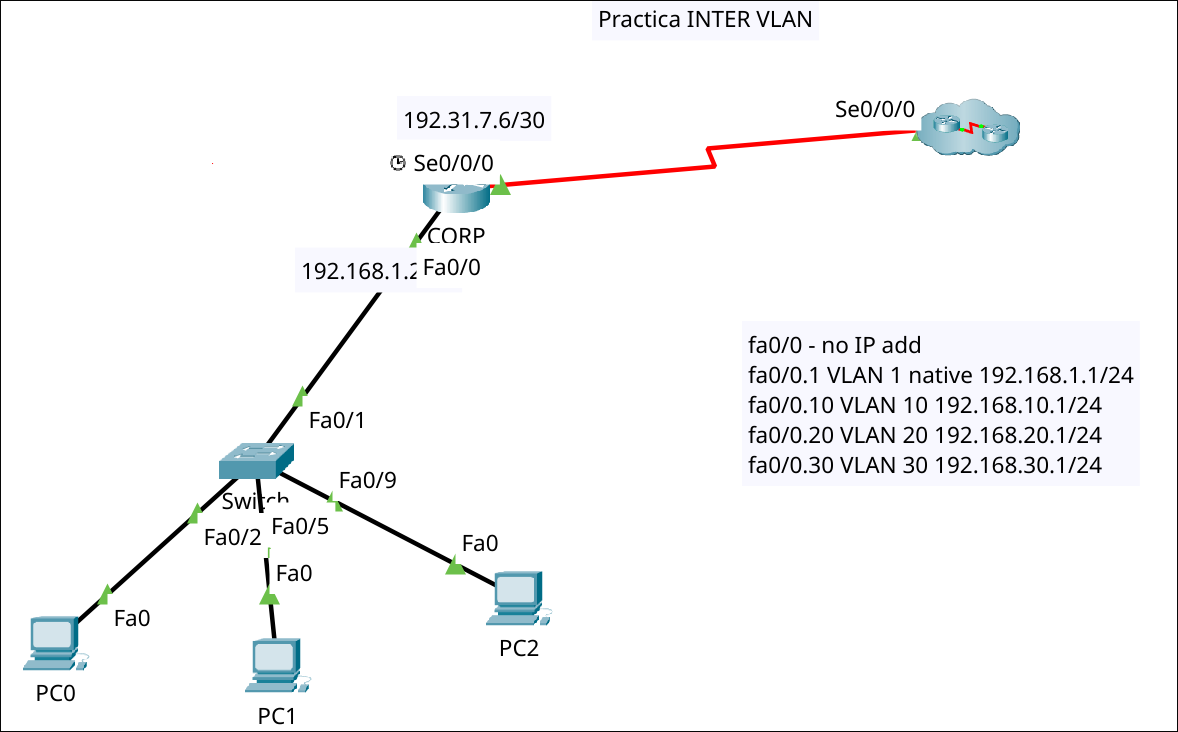
\includegraphics[width=0.7\textwidth]{swappy-20240428-004521.png}
\end{figure}

\section{Información de las VLANs}
\subsection{Router CORP}
\begin{figure}[H]
    \centering 
    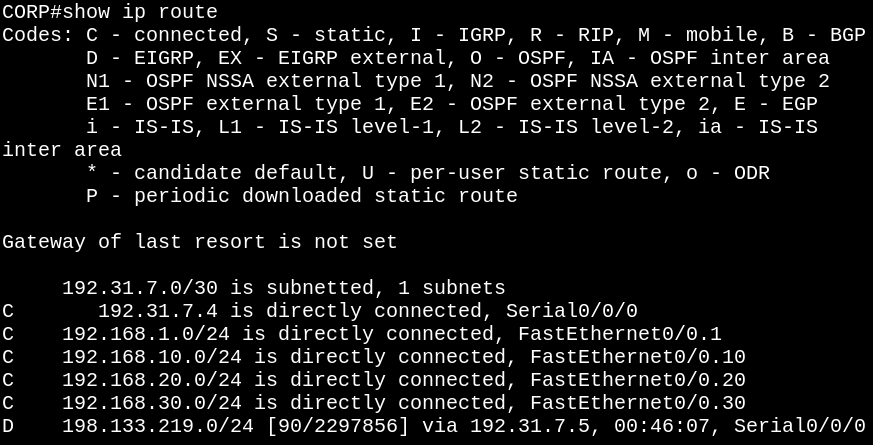
\includegraphics[width=0.6\textwidth]{router.png}
    \vspace{0.3cm}\\ 
    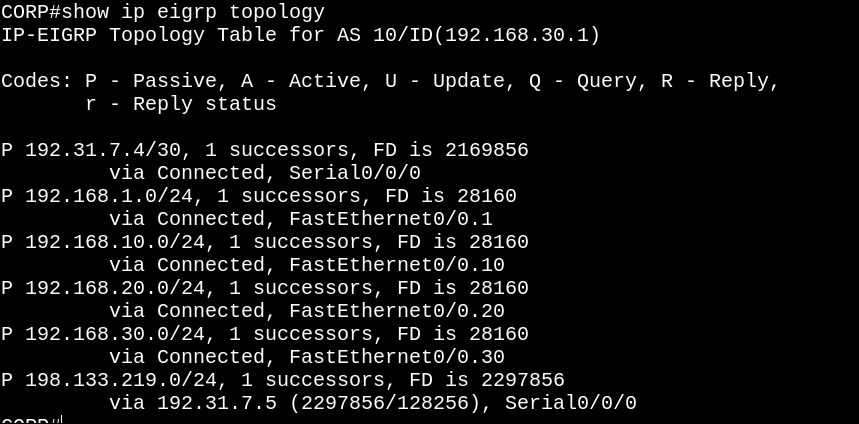
\includegraphics[width=0.6\textwidth]{rout2.png}
    \vspace{0.3cm}\\ 
    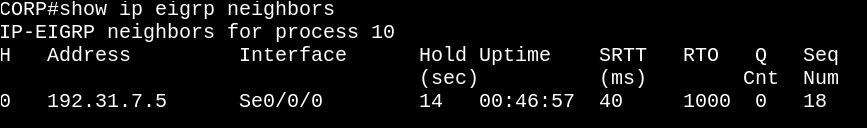
\includegraphics[width=0.6\textwidth]{rout3.png}
\end{figure}
\subsection{Switch}
\begin{figure}[H]
    \centering 
    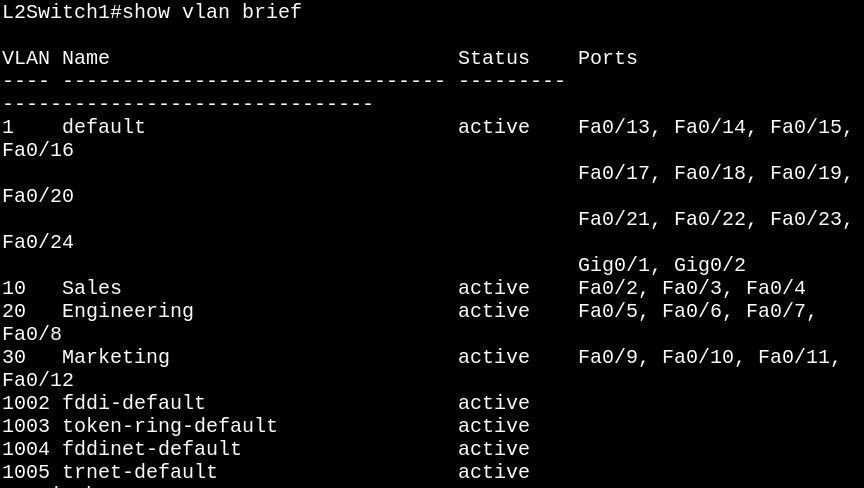
\includegraphics[width=0.6\textwidth]{s1.png}
    \vspace{0.3cm}\\ 
    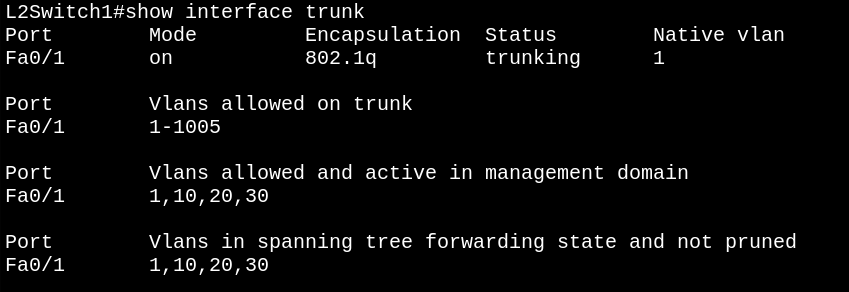
\includegraphics[width=0.6\textwidth]{s2.png}
    \vspace{0.3cm}\\ 
    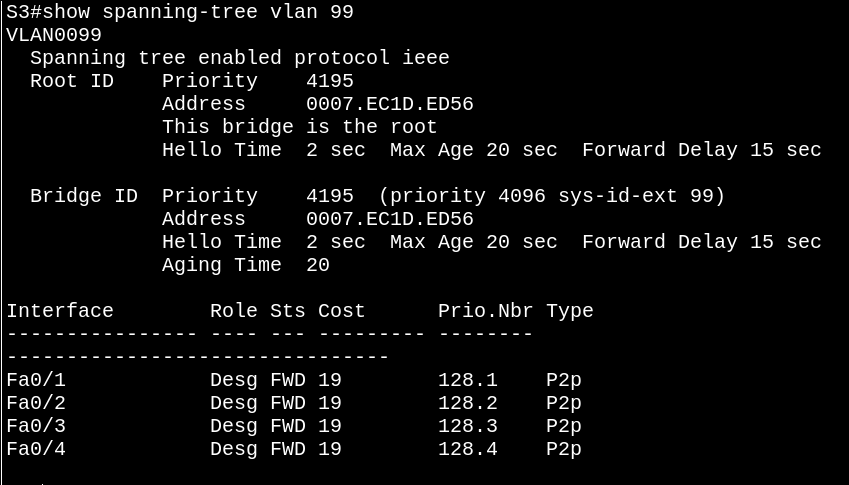
\includegraphics[width=0.6\textwidth]{s3.png}
\end{figure}
\subsection{Prueba de comunicación}
\centering
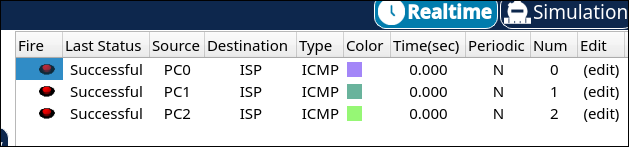
\includegraphics[width=0.6\textwidth]{pruebitsa.png}






\end{sloppypar}
\end{document}